\subsection{\textit{Ad hoc on demand distance vector} - AODV}
O protocolo AODV \'e um protocolo reativo, baseado em vetor de dist\^ancias, e pode ser considerado como uma combina\c{c}\~ao de outros dois protocolos, denominados DSR e DSDV. 
O AODV tem a base do DSR, o qual \'e baseado sob demanda, ou seja, descobre rotas somente quando necess\'ario, e utiliza os mecanismos de descoberta de rotas e manuten\c{c}\~ao de rotas.
Entretando, o AODV utiliza a caracter\'istica do DSDV de obrigar todos os n\'os intermedi\'arios a estabelecerem dinamicamente entradas em tabelas de roteamento locais para cada destino ativo.
Cada n\'o tem conhecimento do pr\'oximo salto para alcan\c{c}ar o destino e a dist\^ancia em n\'umero de saltos.
Pode ser considerado como uma vers\~ao melhorada do DSDV, uma ver que seu funcionamento baseado em demanda minimiza o n\'umero de inunda\c{c}\~oes na rede exigido pelo DSDV para cria\c{c}\~ao de rotas.

\subsubsection{Processo de cria\c{c}\~ao de rotas no AODV}
\begin{figure}[H]
	\centering
	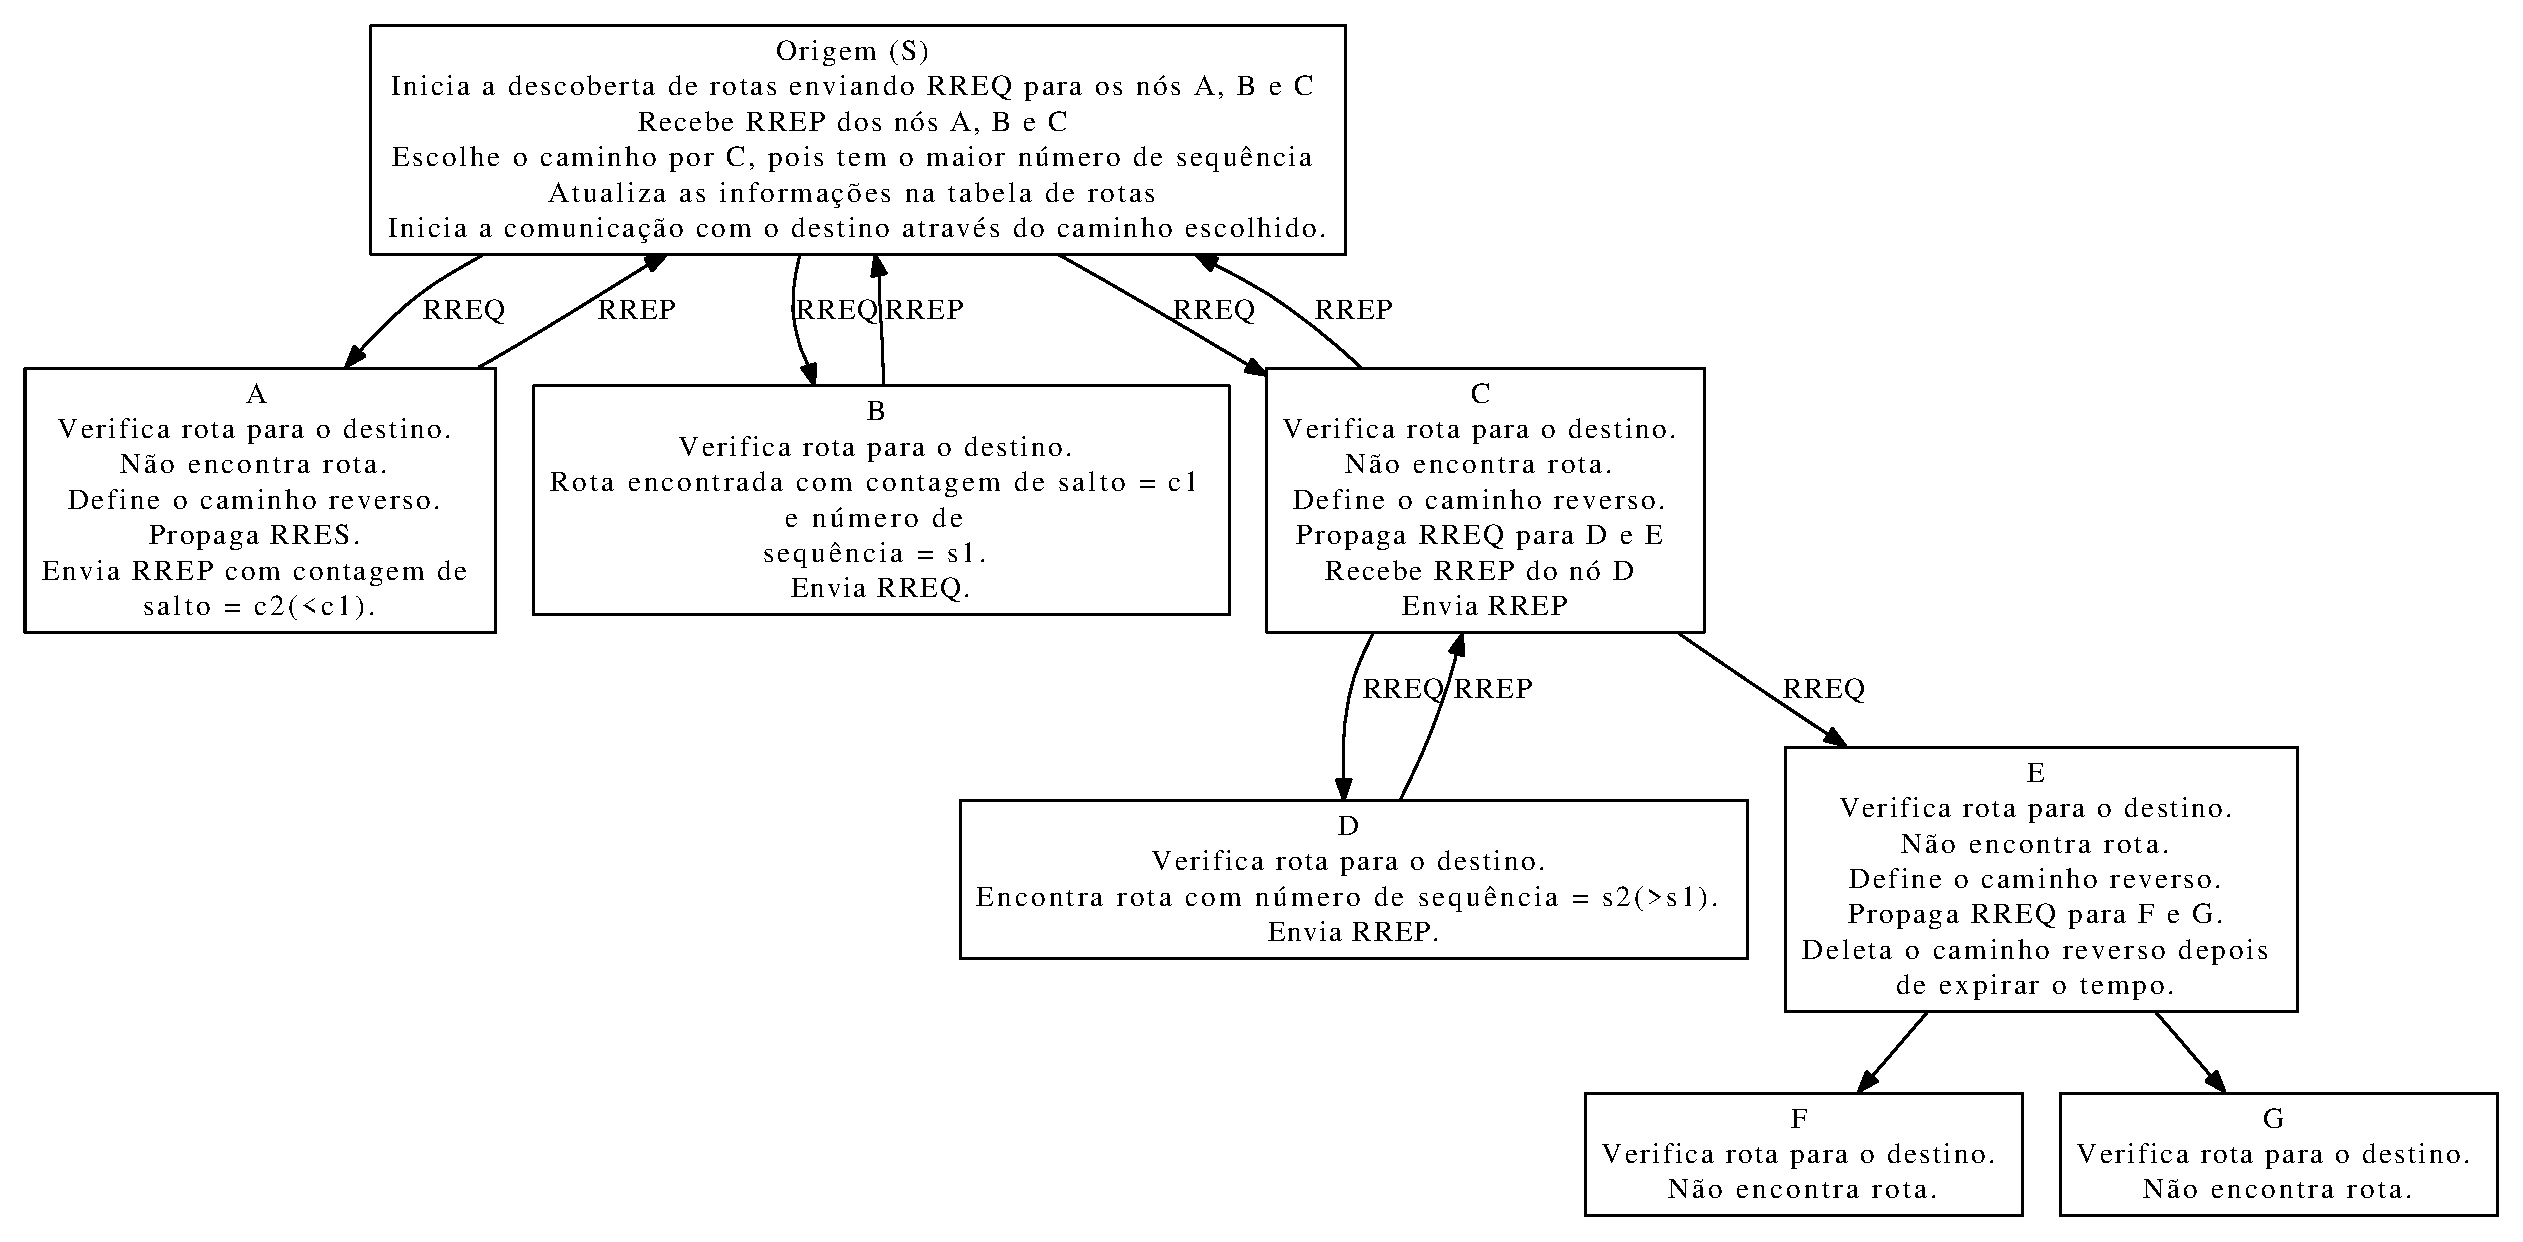
\includegraphics[scale=.43]{aodvOperation.eps}
	\caption{Processo de cria\c{c}\~ao de rotas no AODV \cite{gorantala}}
	\label{figOpAODV}
\end{figure}
Segue passo-a-passo a explica\c{c}\~ao do processo exibido na figura \ref{figOpAODV} acima.
\begin{enumerate}
	\item "Source S" Precisa enviar dados ao destino.
	\item "S" envia RREQ para seus vizinhos "A", "B" e "C".
	\item "B" encontra o caminho em sua tabela de roteamento (com n\'umero de sequ\^encia = s1 e contagem de salto = c1) e envia RREP para "S".
	\item "C" ativa caminho reverso.
	\item "C" redireciona RREQ para seus vizinhos "D" e "E".
	\item "E" ativa caminho reverso.
	\item "E" redireciona RREQ para seus vizinhos "F" e "G".
	\item "E" deleta o caminho reverso ap\'os um per\'iodo de tempo limite, uma vez que n\~ao recebe qualquer RREPs dos n\'os "F" e "G".
	\item "D" encontra o caminho () 
\end{enumerate}

\subsubsection{Vantagens do AODV}
\begin{itemize}
	\item Por causa de sua natureza reativa, o AODV pode lidar com o compartamento di\^amico das redes \textit{ad hoc} \cite{schwingenschlogl}.
	\item Utilizado tanto para \textit{unicasts} quanto \textit{multicasts} com a \textit{flag} 'J' nos pacotes \cite{ramachandranTech}.
\end{itemize}

\subsubsection{Limita\c{c}\~oes e desvantagens do AODV}
\begin{description}
	\item[Necessidade de um meio de propaga\c{c}\~ ao:] O algoritmo necessita que os n\'os no meio da propaga\c{c}\~ ao possam detectar outros 
	\item[N\~ao reutiliza informa\c{c}\~oes de roteamento] O AODV carede de efici\^encia na t\'ecnica de manuten\c{c}\~ao de suas rotas. Informa\c{c}\~oes de roteamento s\~ao sempre atualizadas em cada demanda, inclu\'indo casos comuns de tr\'afego. \cite{ramachandran}
\end{description}
